\section{Descripción del prototipo}
Uno de los objetivos de la realización de este trabajo terminal es permitir al usuario empezar a hacer uso de Big Data de una manera sencilla y sin demasiadas complicaciones. Por lo que se comenzó el desarrollo de un instalador que simplifique el proceso de puesta en marcha del ambiente de análisis de datos.\\

Podría decirse que la utilidad de este prototipo se refleja al comparar el número de pasos que se enuncian en el manual de instalación de \emph{Luminus}, contra el número de pasos que se siguen al utilizar el instalador.\\

En este punto del trabajo terminal, este prototipo se encuentra en una fase aún experimental, sin embargo logra el 
cometido de simplificar el proceso de puesta en marcha.\\

\section{Análisis}
La manera en que se pretende que el instalador simplifique el proceso de instalación es automatizando algunas tareas que de otra forma el usuario tendría que realizar una a una, existiendo así la posibilidad de que éste mismo cometa algún error u omita algún paso, y por lo tanto, el ambiente de análisis de datos no pueda ponerse en funcionamiento.\\
Existen diferentes tecnologías para solventar la instalación y configuración de un conjunto previamente determinado, por ejemplo, Docker.

%referencia donde leiste eso
Sin embargo, para el uso de Big Data se utilizan tecnologías como Apache Hadoop o Apache Spark, mismas que, la instalación y puesta en marcha con Docker se encuentran en fase experimental lo que significa que no es consistente y generaría muchos problemas al momento de querer utilizarlo \cite{generacitapls}.   
\\
Para solventar esto, se decidió hacer uso del Shell Script de Unix/Linux el cual es simplemente un programa que lee los comandos que se teclean y los convierte en una forma mas entendible para el sistema Unix/Linux. También incluye algunas sentencias básicas de programación que permiten: tomar decisiones, realizar ciclos y almacenar valores en variables \cite{Baze}.
\\
Por lo que, dadas las características de Shell a pesar de que este es la forma mas rudimentaria re realizar esta tarea, es la que mejores resultados ofrece para las tecnologías que estamos utilizando.
\\
Utilizar Shell Script por otro lado, implica complicaciones ya que todo lo que el script haga, tendrá que ser programado, y esto implica un gran número de validaciones que de utilizar otras tecnologías no se tendría que realizar, ya que la tecnología por si misma lo resuelve.
\section{Diseño}
La funcionalidad completa del instalador no se encuentra terminada por el momento además de que por ahora solo se tiene contemplada la instalación de los prototipos \nameref{cap:Cap3} y \nameref{cap:Cap4}. 
\\
El instalador, contempla incluir todos los prototipos de este Trabajo Terminal, sin embargo, debido a que aun no se han finalizado todos los prototipos y se desconocen detalles de los mismos por el momento, no se encuentran incluidos en el diseño actual del instalador.
\\
En el diagrama de flujo que se muestra en la figura \ref{fig:diagramaFlujo} se puede apreciar el diseño actual del instalador.
\begin{figure}[!htbp]
	\hypertarget{fig:diagramaFlujo}{\hspace{1pt}}
	\begin{center}
		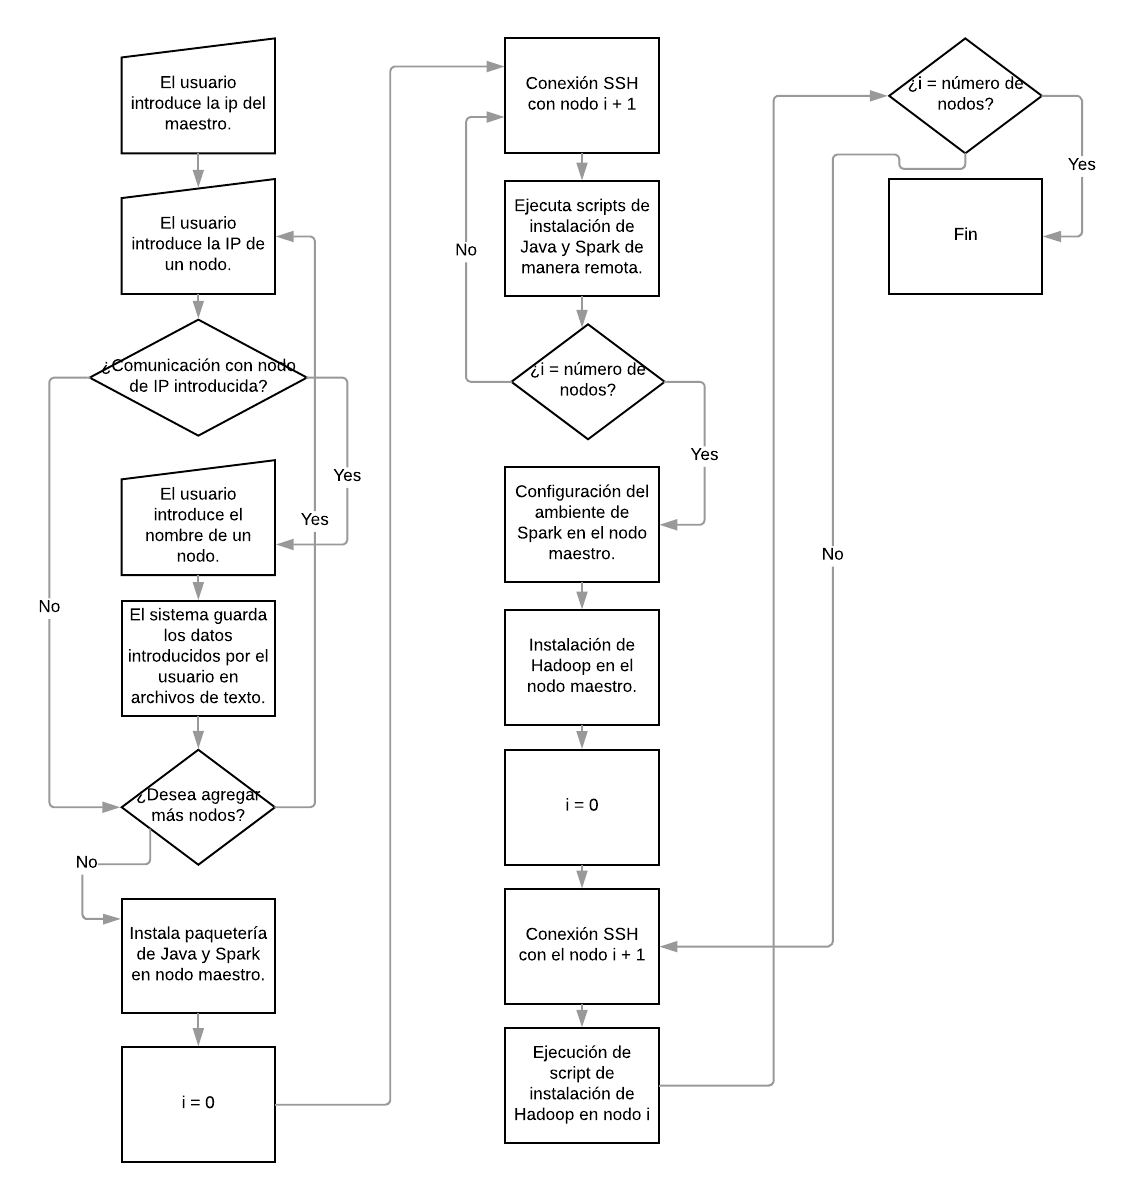
\includegraphics[width=.9\textwidth]{capitulo5/images/diagramaFlujo.png}
		\caption{Fechas de registro en el archivo de resultados}
		\label{fig:diagramaFlujo}
	\end{center}
\end{figure}
\newpage
Como se puede ver en el mismo los pasos de instalación y configuración de las tecnologías se lleva a cabo de igual forma como lo haría el manual de instalación de Luminus, sin embargo se busca que no se haga ninguna configuración directamente sobre los nodos de datos/replica por lo que se pide la dirección IP de los mismos. 
\\
Para que el nodo maestro pueda comunicarse remotamente a los nodos de datos/replica y realizar las instalaciones y configuraciones pertinentes.
\\
Se puede ver como las entradas y salidas del diagrama de flujo con respecto a la intervención del usuario en el manual de instalación actual de Luminus, disminuyen demasiado.
\section{Desarrollo}
El codigo fuente se escribio en Shell Script este contiene los siguientes pasos que se enuncian en el instalador de Luminus.
\begin{verbatim}
1 Instalación de Apache Spark en el nodo
	1.1. Instalación de la paquetería de java 
	1.2. Instalación de la paquetería de SSH	
		1.2.1. Configuración
		1.2.2. Conexión
	1.3. Instalación de Spark
	1.3.1. Configuración maestro

2. Instalación de Apache Spark en los nodos de datos
	2.1. Instalación de la paquetería de java en los nodos de datos
	2.2. Instalación de la paquetería de SSH en los nodos de datos
	2.3. Instalación de Spark en los nodos de datos
		2.3.1. Configuración 
3. Puesta en funcionamiento
	3.1. Configuraciones para poner en funcionamiento Apache Spark en la red distribuida
\end{verbatim}
Las cuales nos permitirán instalar Apache Spark para permitir la conexión entre los nodos de datos/replica y el maestro haciendo uso de una red de internet local en la que se encuentren conectados todos los nodos.
\\
Además de contener todas las configuraciones necesarias para tal objetivo.  
\\
El código fuente actual de este desarrollo se puede consultar en el anexo \ref{anexob}.
\\
Con esto, se logro que el usuario final realice menos pasos de los que tendrían que llevarse a cabo si se siguiera el manual de instalación directamente. 
\\
Los repositorios que se utilizan para tal objetivo, son los mismos que los que se enuncian en el manual de instalación. es de nuestro conocimiento que no se puede confiar en que estos repositorios se encuentren disponibles en el momento en que el usuario experto desee realizar la instalación de \emph{Luminus} se buscará la forma de solventar esta problemática.
\section{Pruebas}
Se presenta a continuación un ejemplo de instalación con el proceso actual a seguir por parte del instalador, así como una descripción de los pasos que este ejecuta. 
\\
El instalador será ejecutado solamente desde la máquina que ocupe el rol de nodo maestro de la red distribuida haciendo uso de su terminal con privilegios de super usuario y ejecutando el siguiente comando. 
\\
\begin{verbatim}
./lum-ins.sh
\end{verbatim}
Éste preguntará al usuario por la IP del nodo maestro. Luego preguntará por las IPs de los nodos que conformarán la red distribuida. Cada que el usuario introduzca una IP, el prototipo hará un ping para comprobar si hay conexión con el nodo cuya IP se desea agregar a la red distribuida. Si hay respuesta por parte del nodo en cuestión, se procede a almacenar ese dato en un archivo y se le pregunta al usuario si desea agregar otro nodo. Si su respuesta es afirmativa, este proceso se repite. 
\\
El instalador, es capaz de detectar cuando la IP introducida no corresponde a un Host que se encuentre dentro de la red local y notifica al usuario experto de esto, como se muestra en la figura \ref{fig:hostnoencontrado}, sin embargo, la salida cuando se puede encontrar el host es diferente, como se puede observar en la figura \ref{fig:hostencontrado}.
\\

\begin{figure}[H]
	\hypertarget{fig:hostnoencontrado}{\hspace{1pt}}
	\begin{center}	
		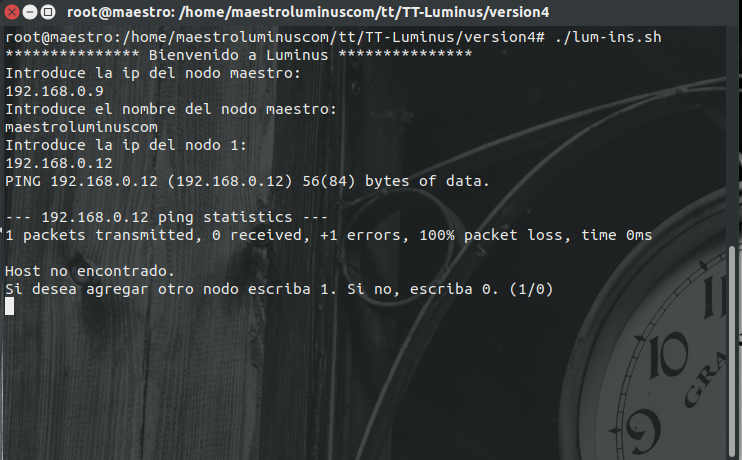
\includegraphics[width=.7\textwidth]{capitulo5/images/hostnoencontrado.png}
		\caption{El usuario introdujo la IP de un host no encontrado.}
	\end{center}
	\label{fig:hostnoencontrado}
\end{figure}

\begin{figure}[H]
	\hypertarget{fig:hostencontrado}{\hspace{1pt}}
	\begin{center}	
		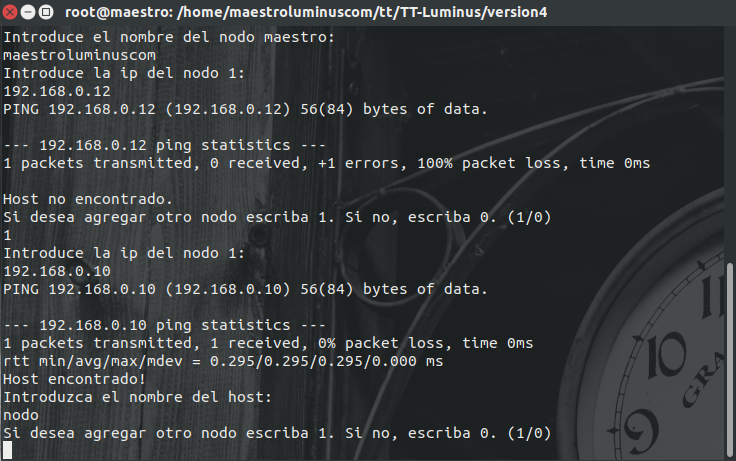
\includegraphics[width=.7\textwidth]{capitulo5/images/hostencontrado.png}
		\caption{El usuario introdujo la IP de un host encontrado.}
	\end{center}
	\label{fig:hostencontrado}
\end{figure}

Posteriormente, cuando ya no se deseen agregar más nodos, el instalador ejecutará varios scripts de instalación en el nodo maestro, desde donde fue ejecutado proceso que puede ser observado en la imagen \ref{fig:instalacion}.\\

\begin{figure}[H]
	\hypertarget{fig:instalacion}{\hspace{1pt}}
	\begin{center}	
		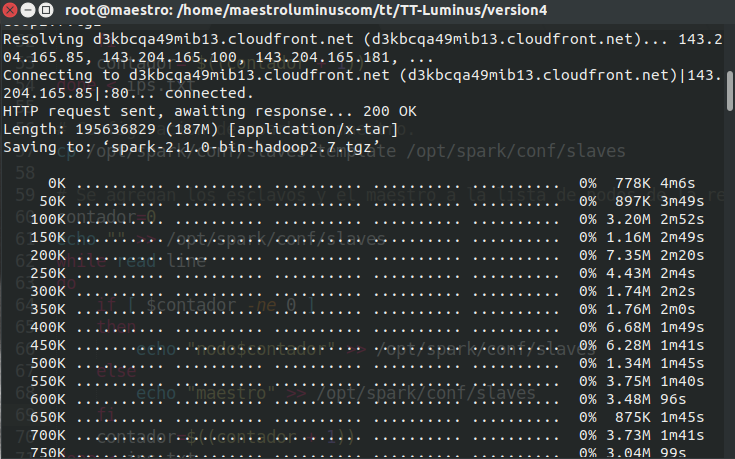
\includegraphics[width=.7\textwidth]{capitulo5/images/instalacion.png}
		\caption{Comienza el proceso de instalación.}
	\end{center}
	\label{fig:instalacion}
\end{figure}

Estos scripts instalarán las tecnologías necesarias para que \emph{Luminus} pueda funcionar de manera adecuada. Estas tecnologías son las siguientes:\\

\begin{enumerate}
	\item SSH. \\
	\item Java.\\
	\item Scala.\\
	\item Spark.\\
\end{enumerate}

Después se procede a establecer conexiones SSH con los nodos de la red. Mediante SSH se ejecutan los mismos scripts que se ejecutaron en el nodo maestro pero de manera remota, es decir, sin la necesidad de tener almacenado el script en el nodo donde se va a iniciar la puesta en marcha del ambiente de análisis de datos.\\

Posteriormente se configura Spark en el nodo maestro, es decir, se asignan roles a los nodos de la red que introdujo el usuario al sistema en un principio.\\

Finalmente se realiza la instalación y configuración de Hadoop en el nodo maestro. Y por último en los nodos de datos/replica.

Una vez que este proceso de instalación finaliza se tiene instalado los prototipos \nameref{cap:Cap3} y \nameref{cap:Cap4} los cuales tendrán todas las configuraciones necesarias para que luminus pueda funcionar correctamente.

